\section{顕微光学系に関して}
\subsection{光源とディフューザー}
本実験には白熱電球を用いた光源を用いた。この光源からの光はそのままでは拡散するので、ファイバーを通してコリメータで平行光に直した。この平行光をビームスプリッタや対物レンズ等を通して試料に入射したところ、図\ref{fig:without_diffuser}のようにまだら模様(スペックルパターン)が見て取れた。
この模様は入射光がコヒーレンスにより干渉してできるものである。この模様の効果を抑えるためには入射光の空間コヒーレンスを小さくする工夫が効果的である。

筆者は入射光のコヒーレンスを小さくするため光学系にEdmund社製のホログラフィックディフューザー(\#47-991/拡散角度$1^\circ$)を導入した。その結果、図\ref{fig:with_diffuser}のように入射光強度の一様な分布が得られた。
キムワイプの切れ端を光路中に挿入しても同様の効果が得られるが、強度が大きく落ち込んでしまい拡散角も大きいことに注意する。
\begin{figure}[htb]]
 \begin{minipage}{0.5\hsize}
  \begin{center}
   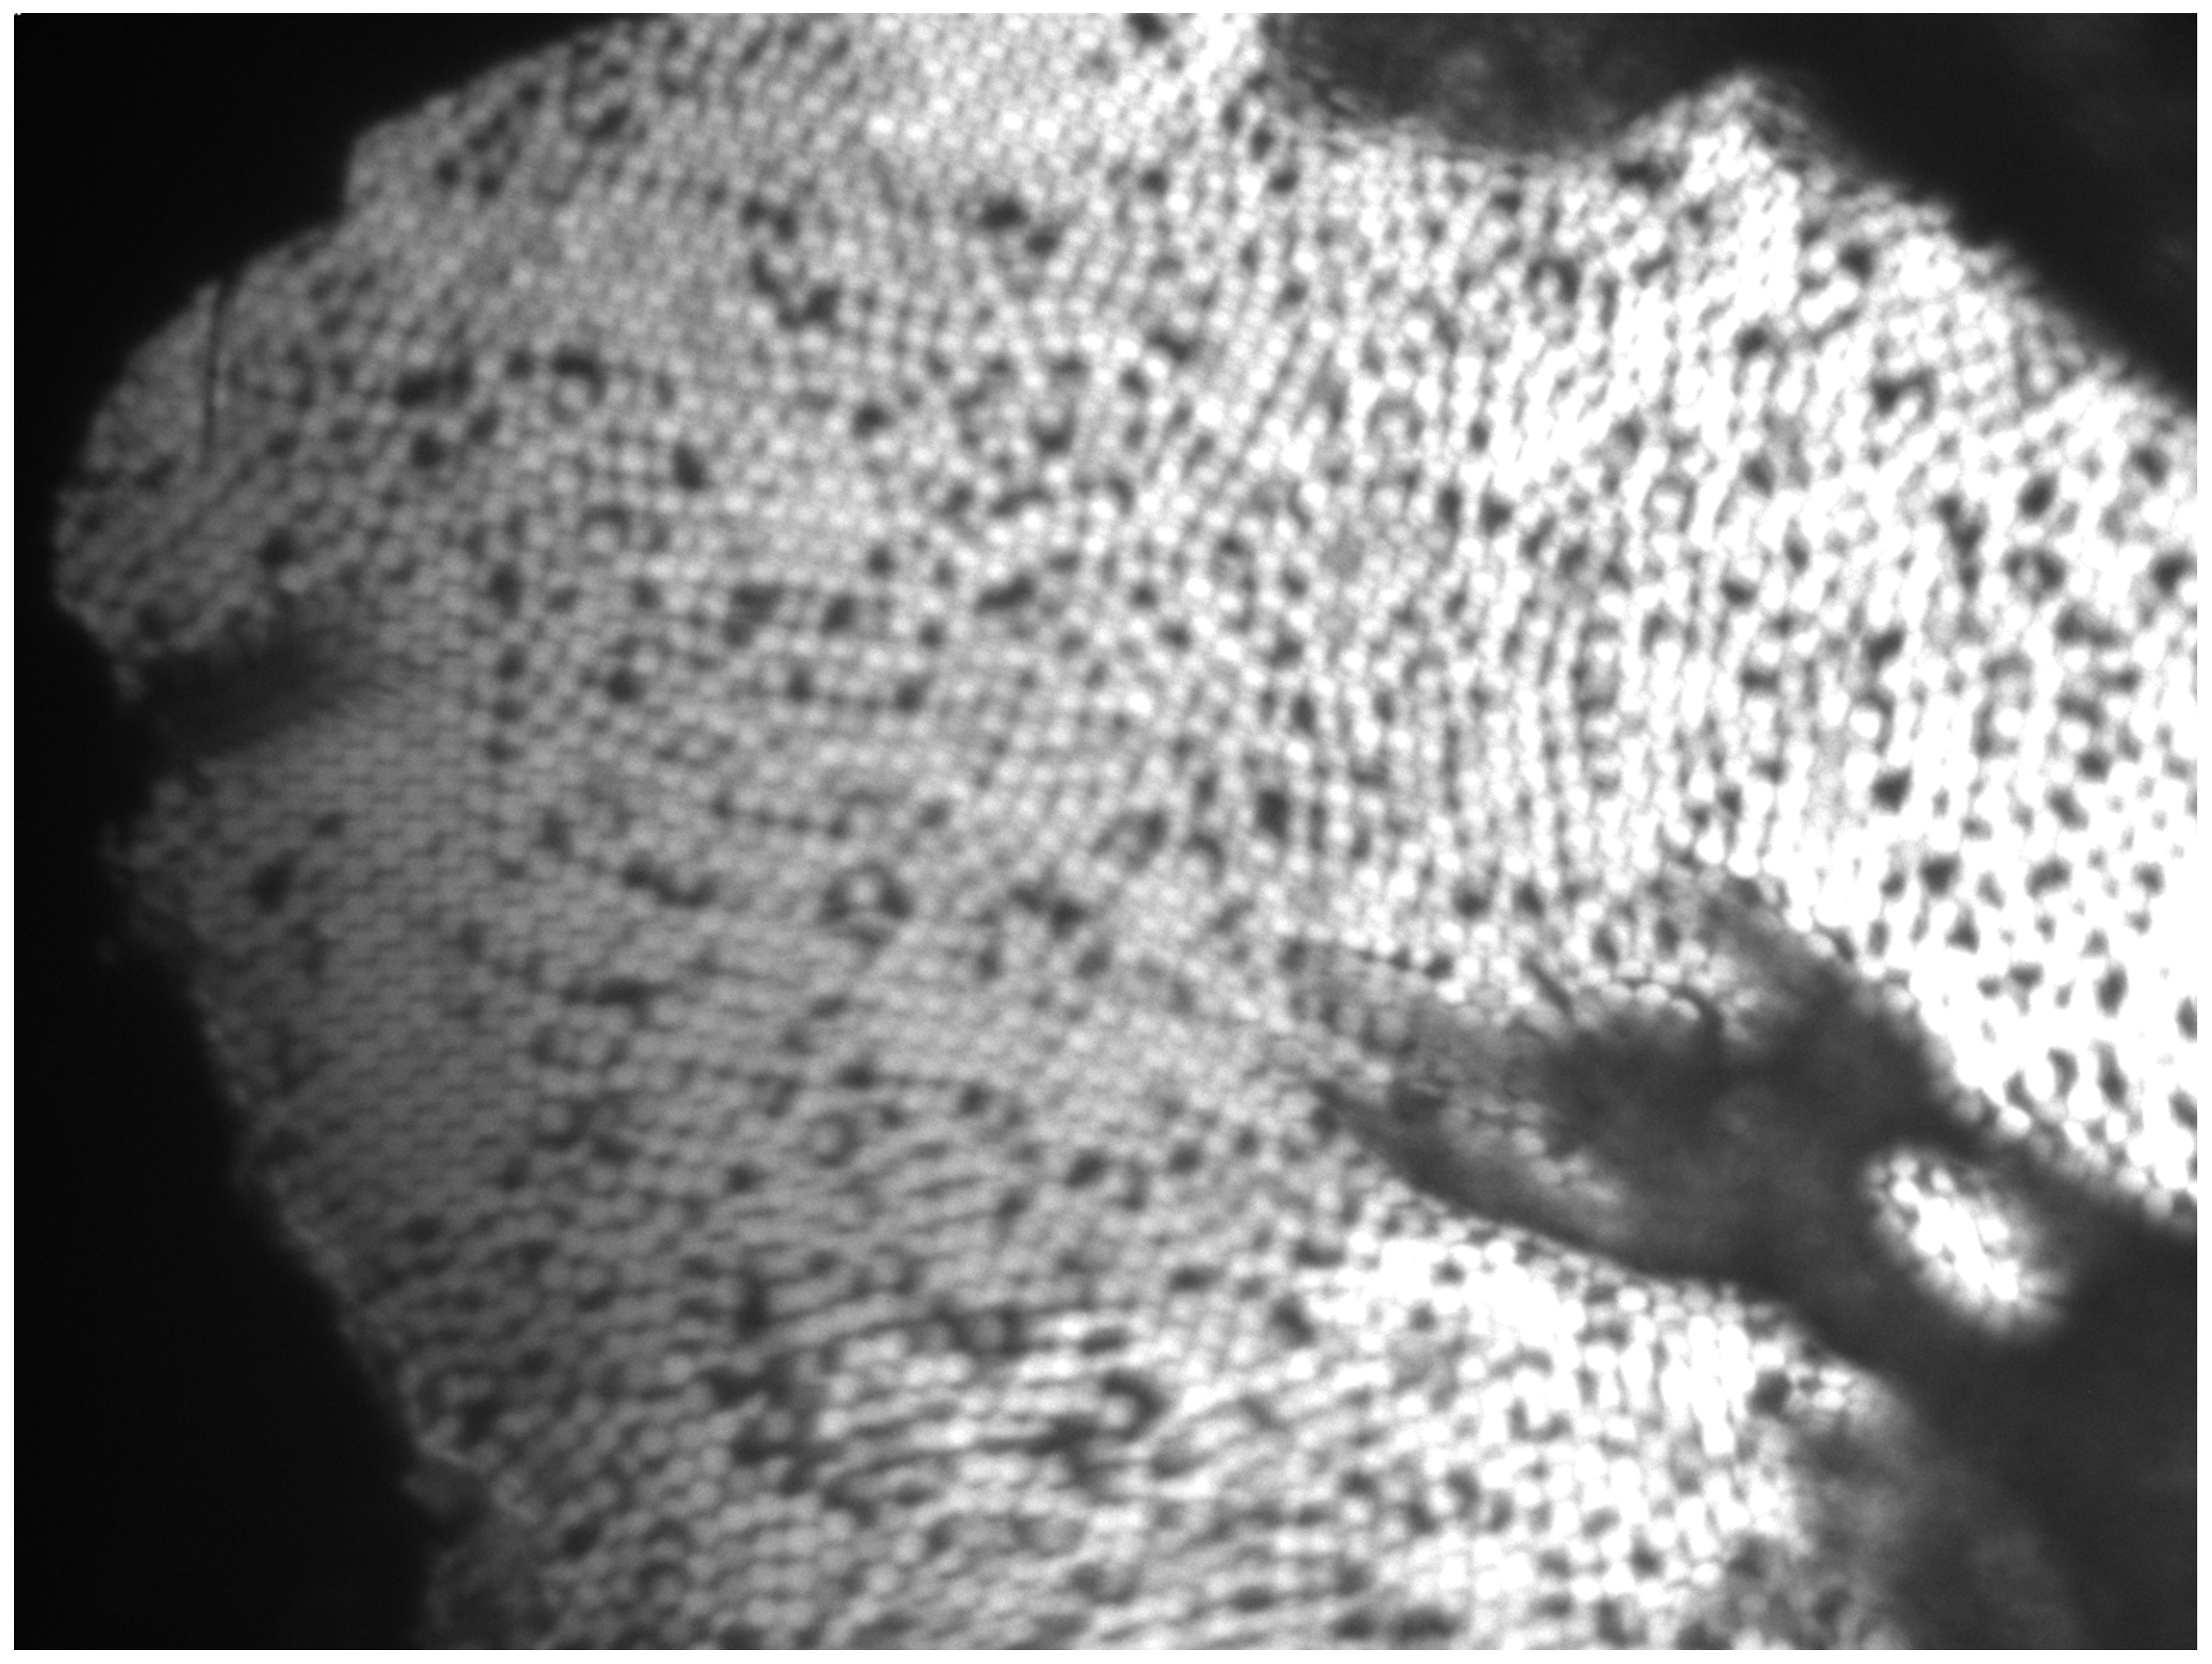
\includegraphics[width=70mm]{without_diffuser.eps}
  \end{center}
  \caption{ディフューザーなし}
  \label{fig:without_diffuser}
 \end{minipage}
 \begin{minipage}{0.5\hsize}
  \begin{center}
   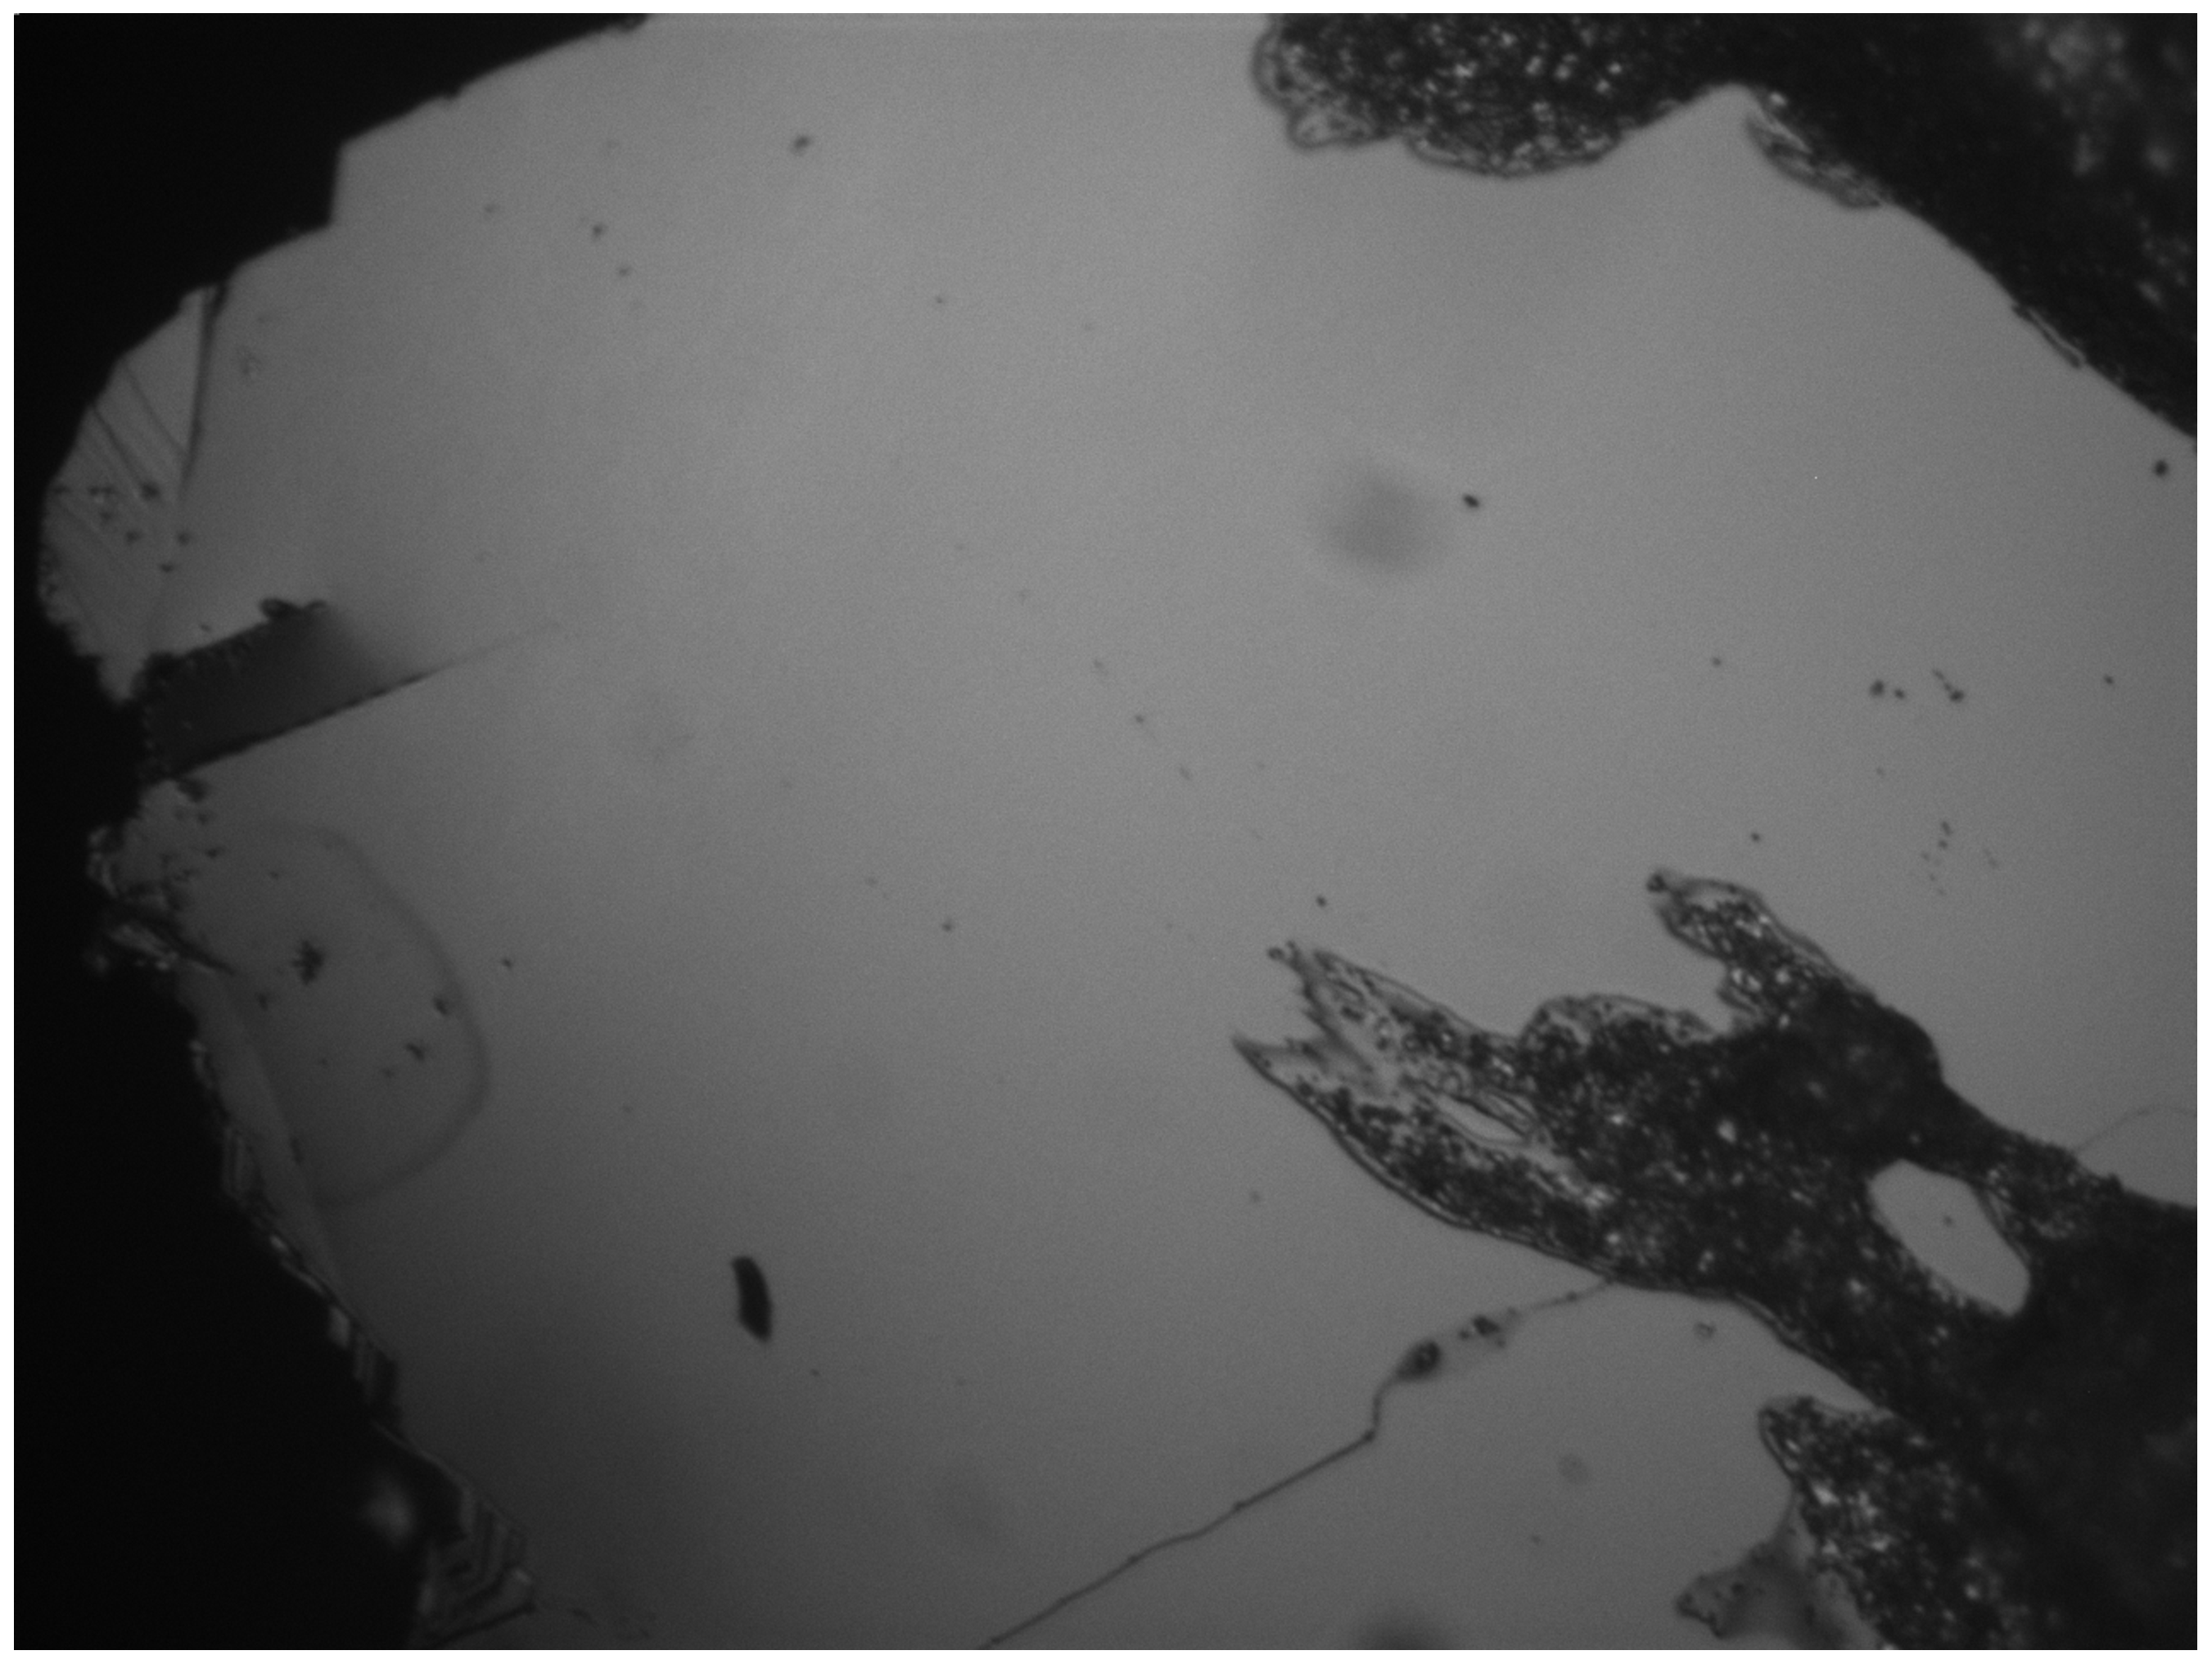
\includegraphics[width=70mm]{with_diffuser.eps}
  \end{center}
  \caption{ディフューザーあり}
  \label{fig:with_diffuser}
 \end{minipage}
\end{figure}

\subsection{非偏光ビームスプリッタの偏光依存性の評価}
\label{seq:BS_characterization}
本節では非偏光ビームスプリッタ(Thorlabs社製\#BSW41-532)の、偏光依存性に関して議論する。

まずビームスプリッタを光が透過する場合に関して、p偏光の透過率とs偏光の透過率を独立に評価し、さらにp偏光の透過光とs偏光の透過光の間についた位相差を評価した。
そのために図\ref{fig:schematics_BS_T2}のような光学系を構成した。光源側の偏光子の偏光軸は鉛直方向と水平方向、鉛直方向に対して45度傾けた角度にとった。偏光軸の角度それぞれに対して検光子を回転させながら、CCDに入る信号の平均強度をプロットしたものが図\ref{fig:BS_T2}である(データ点)。さらにデータ点からビームスプリッタのp偏光の透過率$t_p$とs偏光の透過率$t_s$、p偏光とs偏光の間につく位相差$\phi_t$を推定した。推定は非線形最小二乗法により、解析にはMicrosoft社Excelのソルバーを用いた。その推定した$t_p,t_s,\phi_t$を用いてデータ点をフィッティングした曲線を図\ref{fig:BS_T2}に示す。
p偏光の透過率とs偏光の透過率の比は$t_p/t_s=1.10$で、p偏光とs偏光の間につく位相差は$\phi_t=147^\circ$と推定した。

次にビームスプリッタで光が反射される場合に関しても同様に、p偏光の反射率とs偏光の反射率、p偏光とs偏光の反射光の間についた位相差を評価した。
そのために図\ref{fig:schematics_BS_R}のような光学系を構成した。光源側の偏光子の偏光軸は鉛直方向と水平方向、鉛直方向に対して45度傾けた角度にとった。偏光軸の角度それぞれに対して検光子を回転させながら、CCDに入る信号の平均強度をプロットしたものが図\ref{fig:BS_R}である(データ点)。さらにデータ点に対して、p偏光の反射率$r_p$とs偏光の反射率$r_s$、p偏光とs偏光の間につく位相差$\phi_r$を推定した。推定した$r_p,r_s,\phi_r$を用いたデータ点をフィッティングした曲線を図\ref{fig:BS_R}に示す。
p偏光の透過率とs偏光の透過率の比は$r_p/r_s=1.04$で、p偏光とs偏光の間につく位相差は$\phi_r=24^\circ$と推定した。

最後に図\ref{fig:schematics_BS_T2R}のように、透過と反射が一度ずつあるような光学系で、p偏光の透過率と反射率の積、s偏光の透過率と反射率の積、p偏光とs偏光の間についた位相差を評価した。光源側の偏光子の偏光軸は鉛直方向と水平方向、鉛直方向に対して45度傾けた角度にとった。偏光軸の角度それぞれに対して検光子を回転させながら、CCDに入る信号の平均強度をプロットしたものが図\ref{fig:BS_T2R}である(データ点)。また図\ref{fig:BS_T2R}には、偏光子を取り外した状態で検光子を回転させて信号強度を測定したデータもプロットしてある。データ点に対して、p偏光の透過率と反射率の積$t_pr_p$とs偏光の透過・反射率$t_sr_s$、p偏光とs偏光の間につく位相差$\phi$を推定した。推定した$t_pr_p,t_sr_s,\phi$を用いたデータ点をフィッティングした曲線を図\ref{fig:BS_R}に示す。
p偏光の透過率とs偏光の透過率の比は$t_pr_p/(t_sr_s)=0.99$で、p偏光とs偏光の間につく位相差は$\phi_t=24^\circ$と推定した。

非偏光ビームスプリッタに関して評価した結果を表\ref{tab:BS}にまとめる。

\begin{table}[htb]
  \begin{tabular}{lcrr}
     & 透過 & 反射  & 透過・反射 \\
    透過・反射率の比 & 1.10 & 1.04 & 0.99\\
    位相差($^\circ$) & 147 & 24 &138
    \label{tab:BS}
  \end{tabular}
\end{table}

\begin{figure}[htb]
     \begin{minipage}{\hsize}
  \begin{center}
   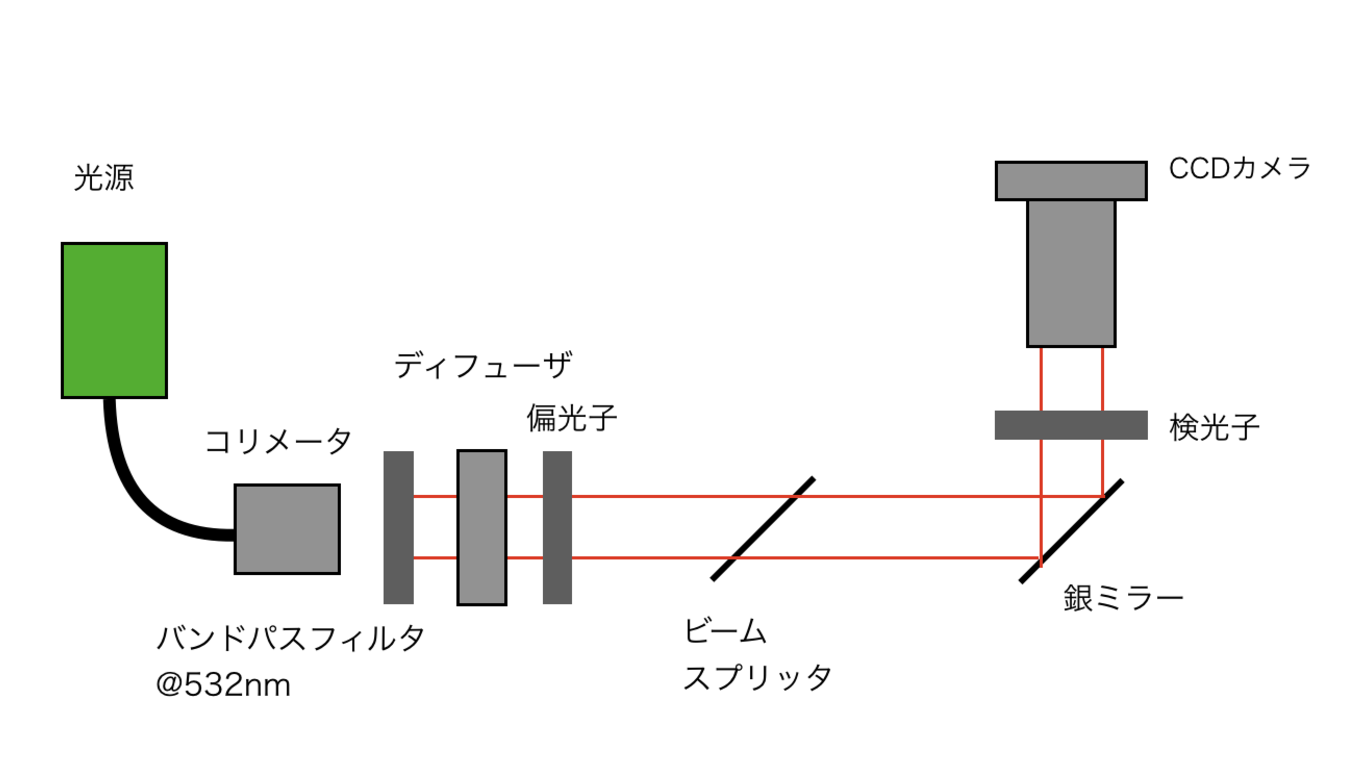
\includegraphics[width=120mm]{schematics_BS_T2.eps}
  \end{center}
  \caption{ビームスプリッタを評価する光学系(透過)}
  \label{fig:schematics_BS_T2}
   \end{minipage}
  \begin{minipage}{\hsize}
  \begin{center}
   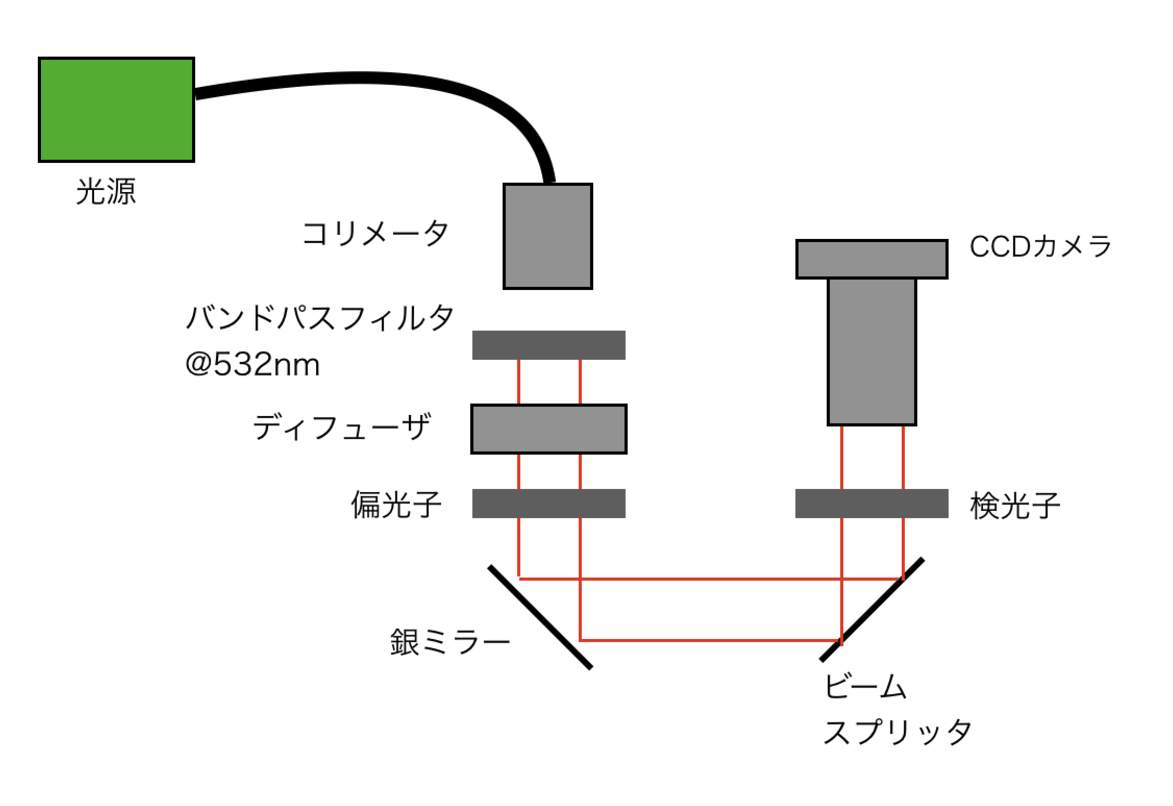
\includegraphics[width=110mm]{schematics_BS_R.eps}
  \end{center}
  \caption{ビームスプリッタを評価する光学系(反射)}
  \label{fig:schematics_BS_R}
   \end{minipage}
     \begin{minipage}{\hsize}
  \begin{center}
   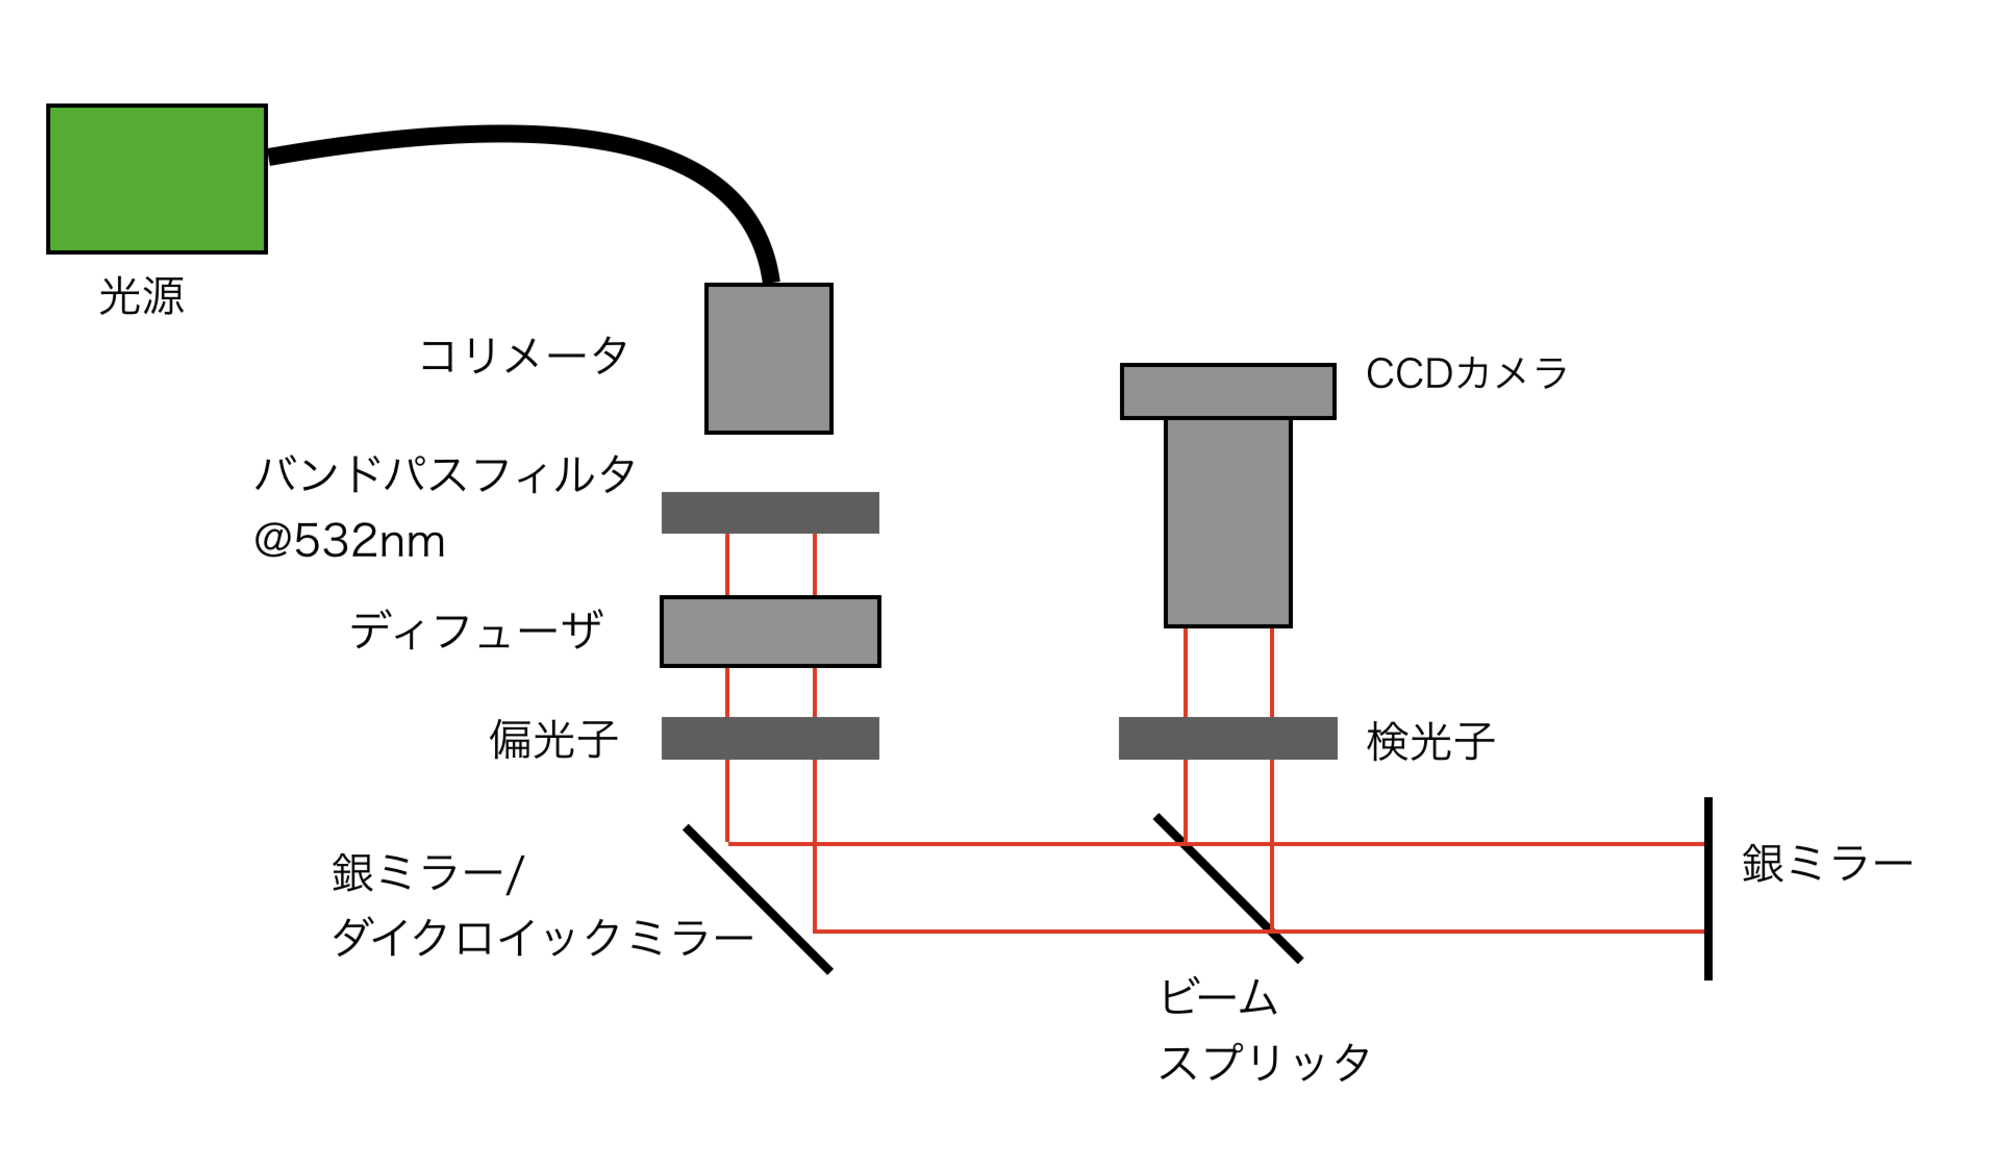
\includegraphics[width=120mm]{schematics_BS_T2R.eps}
  \end{center}
  \caption{ビームスプリッタを評価する光学系(透過・反射)}
  \label{fig:schematics_BS_T2R}
   \end{minipage}
\end{figure}

\begin{figure}[htb]
    \begin{minipage}{\hsize}
  \begin{center}
   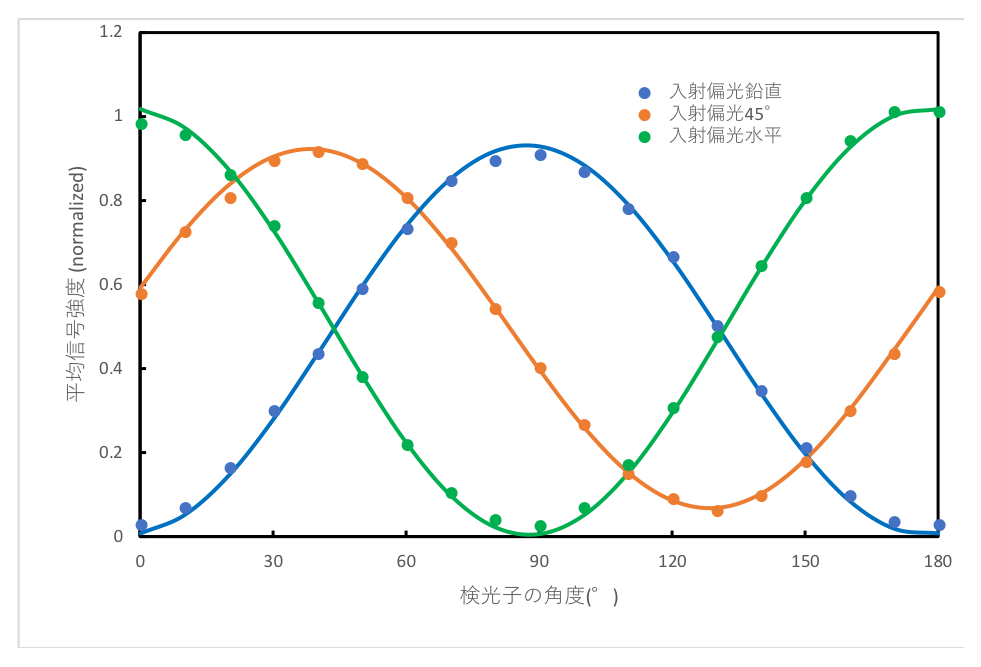
\includegraphics[width=0.7\hsize]{BS_T2.eps}
  \end{center}
  \caption{ビームスプリッタの偏光依存性(透過)}
  \label{fig:BS_T2}
   \end{minipage}
    \begin{minipage}{\hsize}
  \begin{center}
   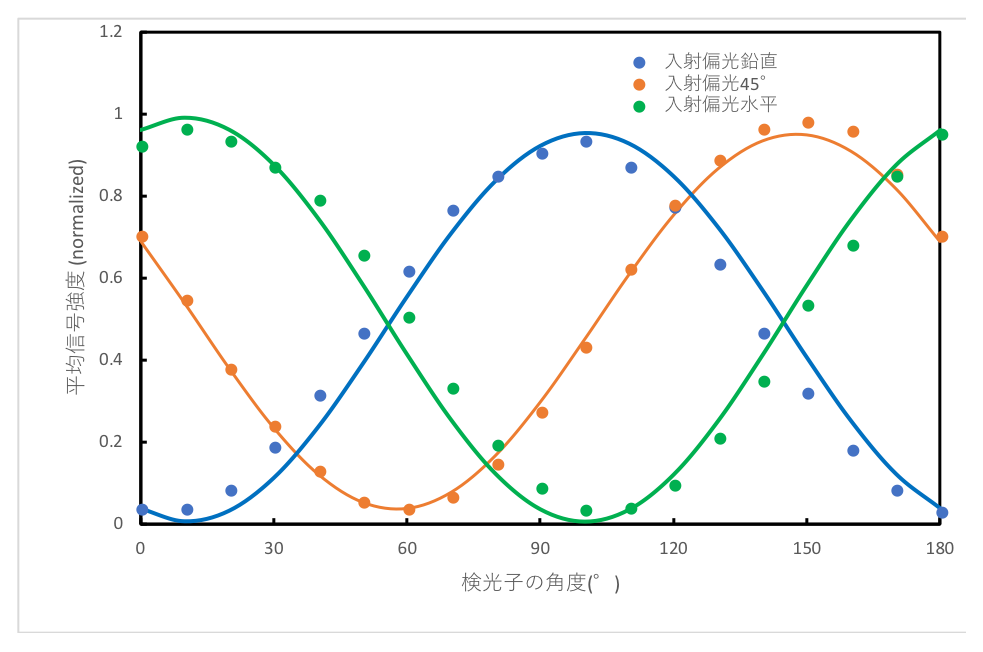
\includegraphics[width=0.7\hsize]{BS_R.eps}
  \end{center}
  \caption{ビームスプリッタの偏光依存性(反射)}
  \label{fig:BS_R}
   \end{minipage}
    \begin{minipage}{\hsize}
  \begin{center}
   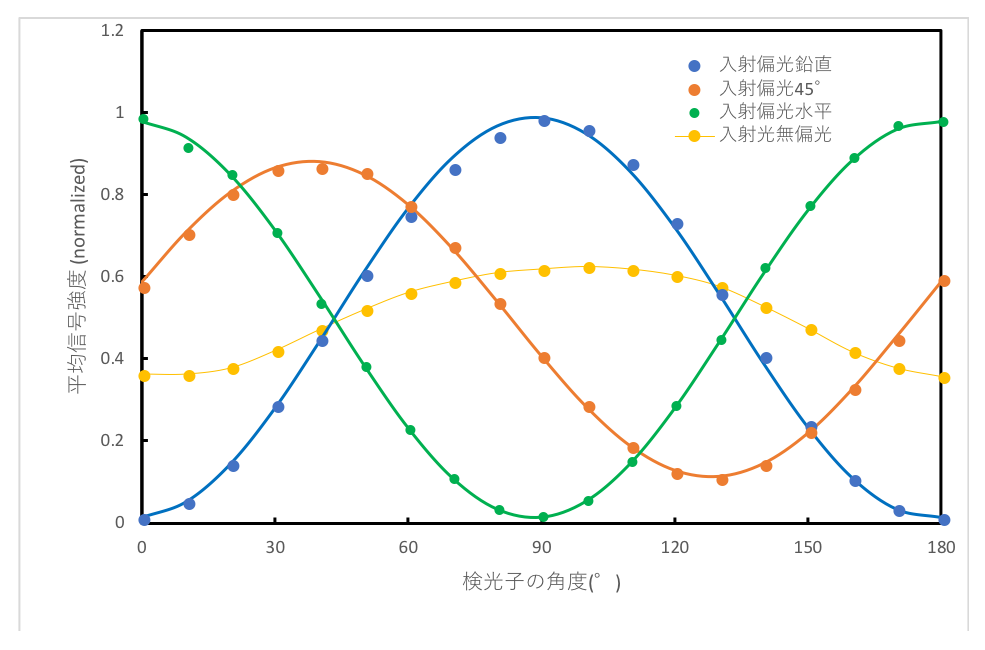
\includegraphics[width=0.7\hsize]{BS_T2R.eps}
  \end{center}
  \caption{ビームスプリッタの偏光依存性(透過・反射)}
  \label{fig:BS_T2R}
   \end{minipage}
\end{figure}


\subsection{顕微光学系の実効的な消光比について}
図\ref{fig:microscope}の光学系で試料の代わりに銀ミラーを置き、偏光子と検光子を垂直に配置したときの信号強度と平行に配置したときの信号強度をそれぞれ測定して、その比(実効的な消光比と呼ぶ)をとるとたかだか10程度だった。すなわち現状の光学系では直交偏光の条件でも、平行偏光の信号成分を精度よく取り除けていない。このとき、直交偏光で試料を顕微鏡像を撮影しても、強度の大きな平行偏光からの寄与がのってしまい、結晶の異方性を観察するのに都合が悪い。

本実験で用いたガラス偏光フィルター(Edmund製\#43-786)は波長532nmで消光比15000程度である。したがって現状で平行偏光の成分を取り除けていないのは、主にビームスプリッタと対物レンズの特性に起因すると筆者は考える。

まずビームスプリッタの寄与に関して述べる。付録\ref{seq:BS_characterization}の結果から、ビームスプリッタ(Thorlabs社製\#BSW41-532)を透過したp偏光とs偏光には位相差がついてしまう。筆者のこれまでの実験では、偏光子の偏光軸を精度よく鉛直・水平方向に出していなかった。実際に付録\ref{seq:BS_characterization}の非線形最小二乗法による解析では、偏光子の偏光軸のアライメントに5度程度の誤差があった可能性が示唆された。 したがってp偏光を入射したつもりでも、実際はビームスプリッタにはp偏光からわずかに傾いた光が入射され、楕円偏光がビームスプリッタから出力されていた。この光学系のアライメントのずれに起因して、顕微光学系の実効的な消光比が小さくなってしまった可能性がある。偏光子の偏光軸を精度よく水平・鉛直方向に出すには、反射率が偏光に依存するビームスプリッタ(Thorlabs製\#BSW-26)で反射される光をCCDで検出し、その結果を解析することが効果的だと筆者は考える。このような偏光子のアライメント方法の改良のもとで、顕微光学系の実効的な消光比はいくらか改善することが見込まれる。

次に顕微光学系の実効的な消光比に対する対物レンズの寄与を評価する実験を行なった。図\ref{fig:microscope}の光学系で試料の代わりに銀ミラーを置き、光源側の偏光子の偏光軸は鉛直方向と水平方向、鉛直方向に対して45度傾けた角度にとった。偏光軸の角度それぞれに対して検光子を回転させながら、CCDに入る信号の平均強度をプロットしたものが図\ref{fig:objective_2}である。図\ref{fig:BS_T2R}のデータを取得した時と比較して、対物レンズを光学系に挿入している点のみが異なる。
対物レンズを挿入しなかったとき(図\ref{fig:BS_T2R})の消光比は73程度だったが、対物レンズ(Mitsutoyo製M Plan Apoシリーズ/倍率x10)を挿入したとき(図\ref{fig:objective_2})の消光比は10程度だった。したがって対物レンズを挿入することで、偏光顕微光学系の実効的な消光比は大きく損なわれることが分かった。

対物レンズを挿入したことで消光比が落ち込む理由は、対物レンズの光軸から離れたところを通る光の一部が偏光方向を回転してしまうことにある。対物レンズの光軸から離れたところで光軸と平行に進む光はレンズの曲面に対して斜めに入射する。斜め入射する光の透過率は偏光に依存するため、透過光の偏光は回転する。また透過率が偏光に依存せず100\%だと仮定しても、対物レンズの光軸から離れたところを通る光の光路は曲げられるため、一般に偏光の方向も変わってしまう。これらの効果により直線偏光を対物レンズに入射しても、集光されて出てくる光の偏光状態は空間的に異なった分布を持つ。対物レンズを用いる現状の光学系で、このような効果の影響を完全に排除することはできない。しかし入射光を対物レンズの光軸付近のみに通し、光軸付近を通った反射光のみ検出すれば、影響を小さくできる。すなわち照明光を空間的に絞ってビームサイズを小さくし、さらに対物レンズの光軸付近を通っってきた反射光のみを検出する工夫が消光比を改善するために効果的である。この工夫は光学系にアイリスを挿入することで簡単に実現できる。すなわち図\ref{fig:microscope3}のような偏光光学系を構成すれば、対物レンズに起因する消光比の悪化を軽減することができると筆者は考える。


\begin{figure}[htb]
  \begin{center}
   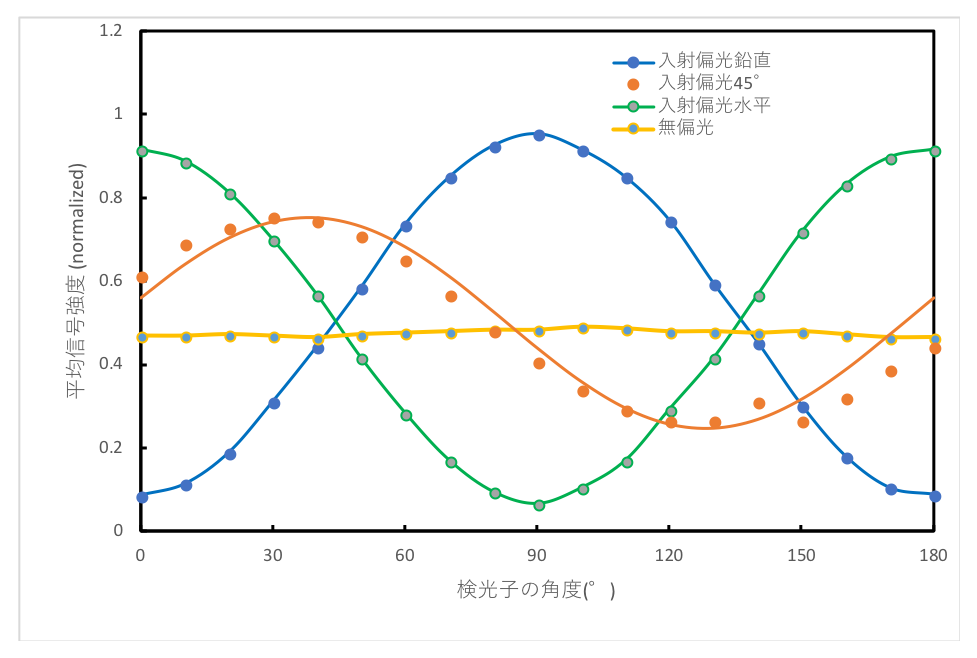
\includegraphics[width=120mm]{objective_2.eps}
  \end{center}
  \caption{顕微光学系の偏光依存性}
  \label{fig:objective_2}
\end{figure}

\begin{figure}[htb]
  \begin{center}
   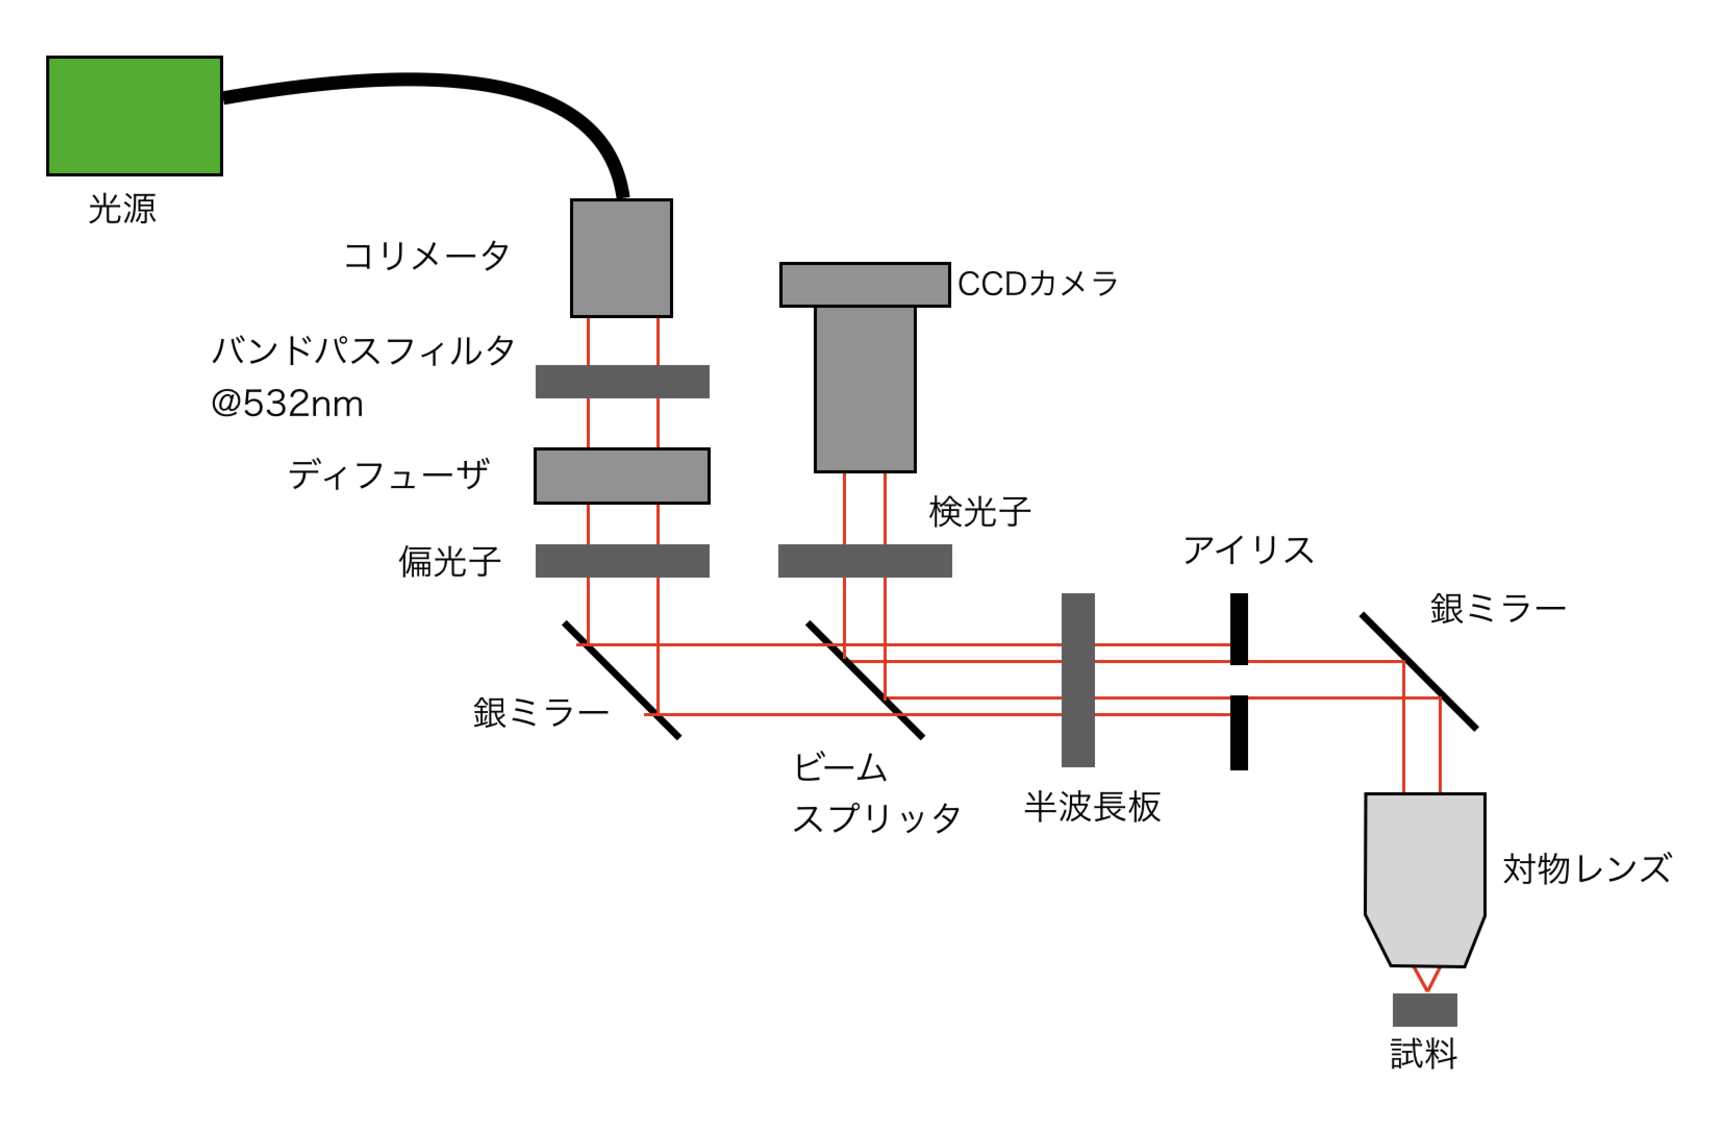
\includegraphics[width=120mm]{microscope3.eps}
  \end{center}
  \caption{改良された偏光顕微光学系の模式図}
  \label{fig:microscope3}
\end{figure}
